%%%%%%%%%%%%%%%%%%%%%%%%%%%%%%%%%%%%%%%%%
% Jacobs Landscape Poster
% LaTeX Template
% Version 1.1 (14/06/14)
%
% Created by:
% Computational Physics and Biophysics Group, Jacobs University
% https://teamwork.jacobs-university.de:8443/confluence/display/CoPandBiG/LaTeX+Poster
% 
% Further modified by:
% Nathaniel Johnston (nathaniel@njohnston.ca)
%
% This template has been downloaded from:
% http://www.LaTeXTemplates.com
%
% License:
% CC BY-NC-SA 3.0 (http://creativecommons.org/licenses/by-nc-sa/3.0/)
%
%%%%%%%%%%%%%%%%%%%%%%%%%%%%%%%%%%%%%%%%%

%---------------------------s-------------------------------------------------------------
%	PACKAGES AND OTHER DOCUMENT CONFIGURATIONS
%----------------------------------------------------------------------------------------

\documentclass[final]{beamer}

\usepackage[scale=1.2]{beamerposter} % Use the beamerposter package for laying out the poster
\usepackage{media9}
\usepackage{subfig}
\usepackage{geometry}

\usetheme{confposter} % Use the confposter theme supplied with this template
\setbeamercolor{title}{fg=blue,bg=white}
\setbeamercolor{block title}{fg=ngreen,bg=white} % Colors of the block titles
\setbeamercolor{block body}{fg=black,bg=white} % Colors of the body of blocks
\setbeamercolor{block alerted title}{fg=white,bg=orange!70} % Colors of the highlighted block titles
\setbeamercolor{block alerted body}{fg=black,bg=orange!10} % Colors of the body of highlighted blocks


% Many more colors are available for use in beamerthemeconfposter.sty

%-----------------------------------------------------------
% Define the column widths and overall poster size
% To set effective sepwid, onecolwid and twocolwid values, first choose how many columns you want and how much separation you want between columns
% In this template, the separation width chosen is 0.024 of the paper width and a 4-column layout
% onecolwid should therefore be (1-(# of columns+1)*sepwid)/# of columns e.g. (1-(4+1)*0.024)/4 = 0.22
% Set twocolwid to be (2*onecolwid)+sepwid = 0.464
% Set threecolwid to be (3*onecolwid)+2*sepwid = 0.708

\newlength{\sepwid}
\newlength{\onecolwid}
\newlength{\twocolwid}
\newlength{\threecolwid}
\setlength{\paperwidth}{48in} % A0 width: 46.8in
\setlength{\paperheight}{36in} % A0 height: 33.1in
\setlength{\sepwid}{0.024\paperwidth} % Separation width (white space) between columns
\setlength{\onecolwid}{0.22\paperwidth} % Width of one column
\setlength{\twocolwid}{0.464\paperwidth} % Width of two columns
\setlength{\threecolwid}{0.708\paperwidth} % Width of three columns
\setlength{\topmargin}{-1.5in} % Reduce the top margin size

%-----------------------------------------------------------



\usepackage{graphicx}  % Required for including images

\usepackage{booktabs} % Top and bottom rules for tables

%----------------------------------------------------------------------------------------
%	TITLE SECTION 
%----------------------------------------------------------------------------------------

\title{Multi instrument music generation using VAE} % Poster title
\author{Saravana Rathinam (saravanr@stanford.edu)} % Author(s)
\institute{SCPD Student, Stanford University} % Institution(s)
%----------------------------------------------------------------------------------------

\begin{document}

\addtobeamertemplate{block end}{}{\vspace*{2ex}} % White space under blocks
\addtobeamertemplate{block alerted end}{}{\vspace*{2ex}} % White space under highlighted (alert) blocks
\addtobeamertemplate{institute}{}{\vspace{-20em}}

\setlength{\belowcaptionskip}{2ex} % White space under figures
\setlength\belowdisplayshortskip{2ex} % White space under equations

\begin{frame}[t] % The whole poster is enclosed in one beamer frame

\begin{columns}[t] % The whole poster consists of three major columns, the second of which is split into two columns twice - the [t] option aligns each column's content to the top

\begin{column}{\sepwid}\end{column} % Empty spacer column

\begin{column}{\onecolwid} % The first column

%----------------------------------------------------------------------------------------
%	OBJECTIVES
%----------------------------------------------------------------------------------------

\begin{alertblock}{Summary}

MIDI format gives a compressed representation of
a Music which may give us a tractable way to generate long melodies. In this project we generate MIDI audio using Variation Auto Encoders (VAE) for multiple instruments. We also generate MIDI sequences given a short begining sequence and let the model fill in the rest using a Conditional-VAE.

\end{alertblock}

\begin{block}{Motivation}

Recent advances in Generative models
for Music generation have shown impressive results. Learning the distribution of music creation may be an intractable problem at the moment.
However one approach we can take is to build tools that serve as an aid in the creative process. If a
musician already has a few ideas in mind on how a song or melody should start, can the problem be
modelled as a conditional generative process where given the start can a model
generate multiple possibilities of how the song can proceed?
\end{block}


%----------------------------------------------------------------------------------------
%	INTRODUCTION
%----------------------------------------------------------------------------------------

\begin{block}{Background Information}

A MIDI sequence can be thought to consist of a list of notes and attributes. Each note has:

\begin{enumerate}
\item \textbf{Pitch}: Frequencey of the note
\item \textbf{Velocity}: Intensity of the note
\item \textbf{Instrument}: The instrument where the note should be played (or synthesized) 
\item \textbf{Program}: A control message that specifies which instrument should be selected to play the note
\item \textbf{Start time}: The start time of the note (seconds)
\item \textbf{End time}: The end time of the note          
\end{enumerate}

The data set consisted of $140944$ midi files obtained from The dataset for the project a combination of the Lakh MIDI Dataset v0.1 \cite{colinlmd} and the MIDI dataset posted at \cite{midiman}. All the MIDI files were encoded into Note Sequences using the Google Magenta library
.



\end{block}
\end{column} % End of the first column


\begin{column}{\sepwid}\end{column} % Empty spacer column

\begin{column}{\twocolwid} % Begin a column which is two columns wide (column 2)

\begin{columns}[t,totalwidth=\twocolwid] % Split up the two columns wide column

\begin{column}{\onecolwid}\vspace{-.6in} % The first column within column 2 (column 2.1)

%------------------------------------------------



%----------------------------------------------------------------------------------------


%----------------------------------------------------------------------------------------
%	MATERIALS
%----------------------------------------------------------------------------------------

\begin{block}{Technical Methods}

The following architectures were tried for controllable generation:

\begin{itemize}
\item Variation Auto Encoder (VAE) with a single Encoder Decoder
\item Beta VAE with $\beta \in [0, 100]$
\item VAE with single Encoder and multiple Decoder sharing $Z$ space
\end{itemize}

\begin{figure}
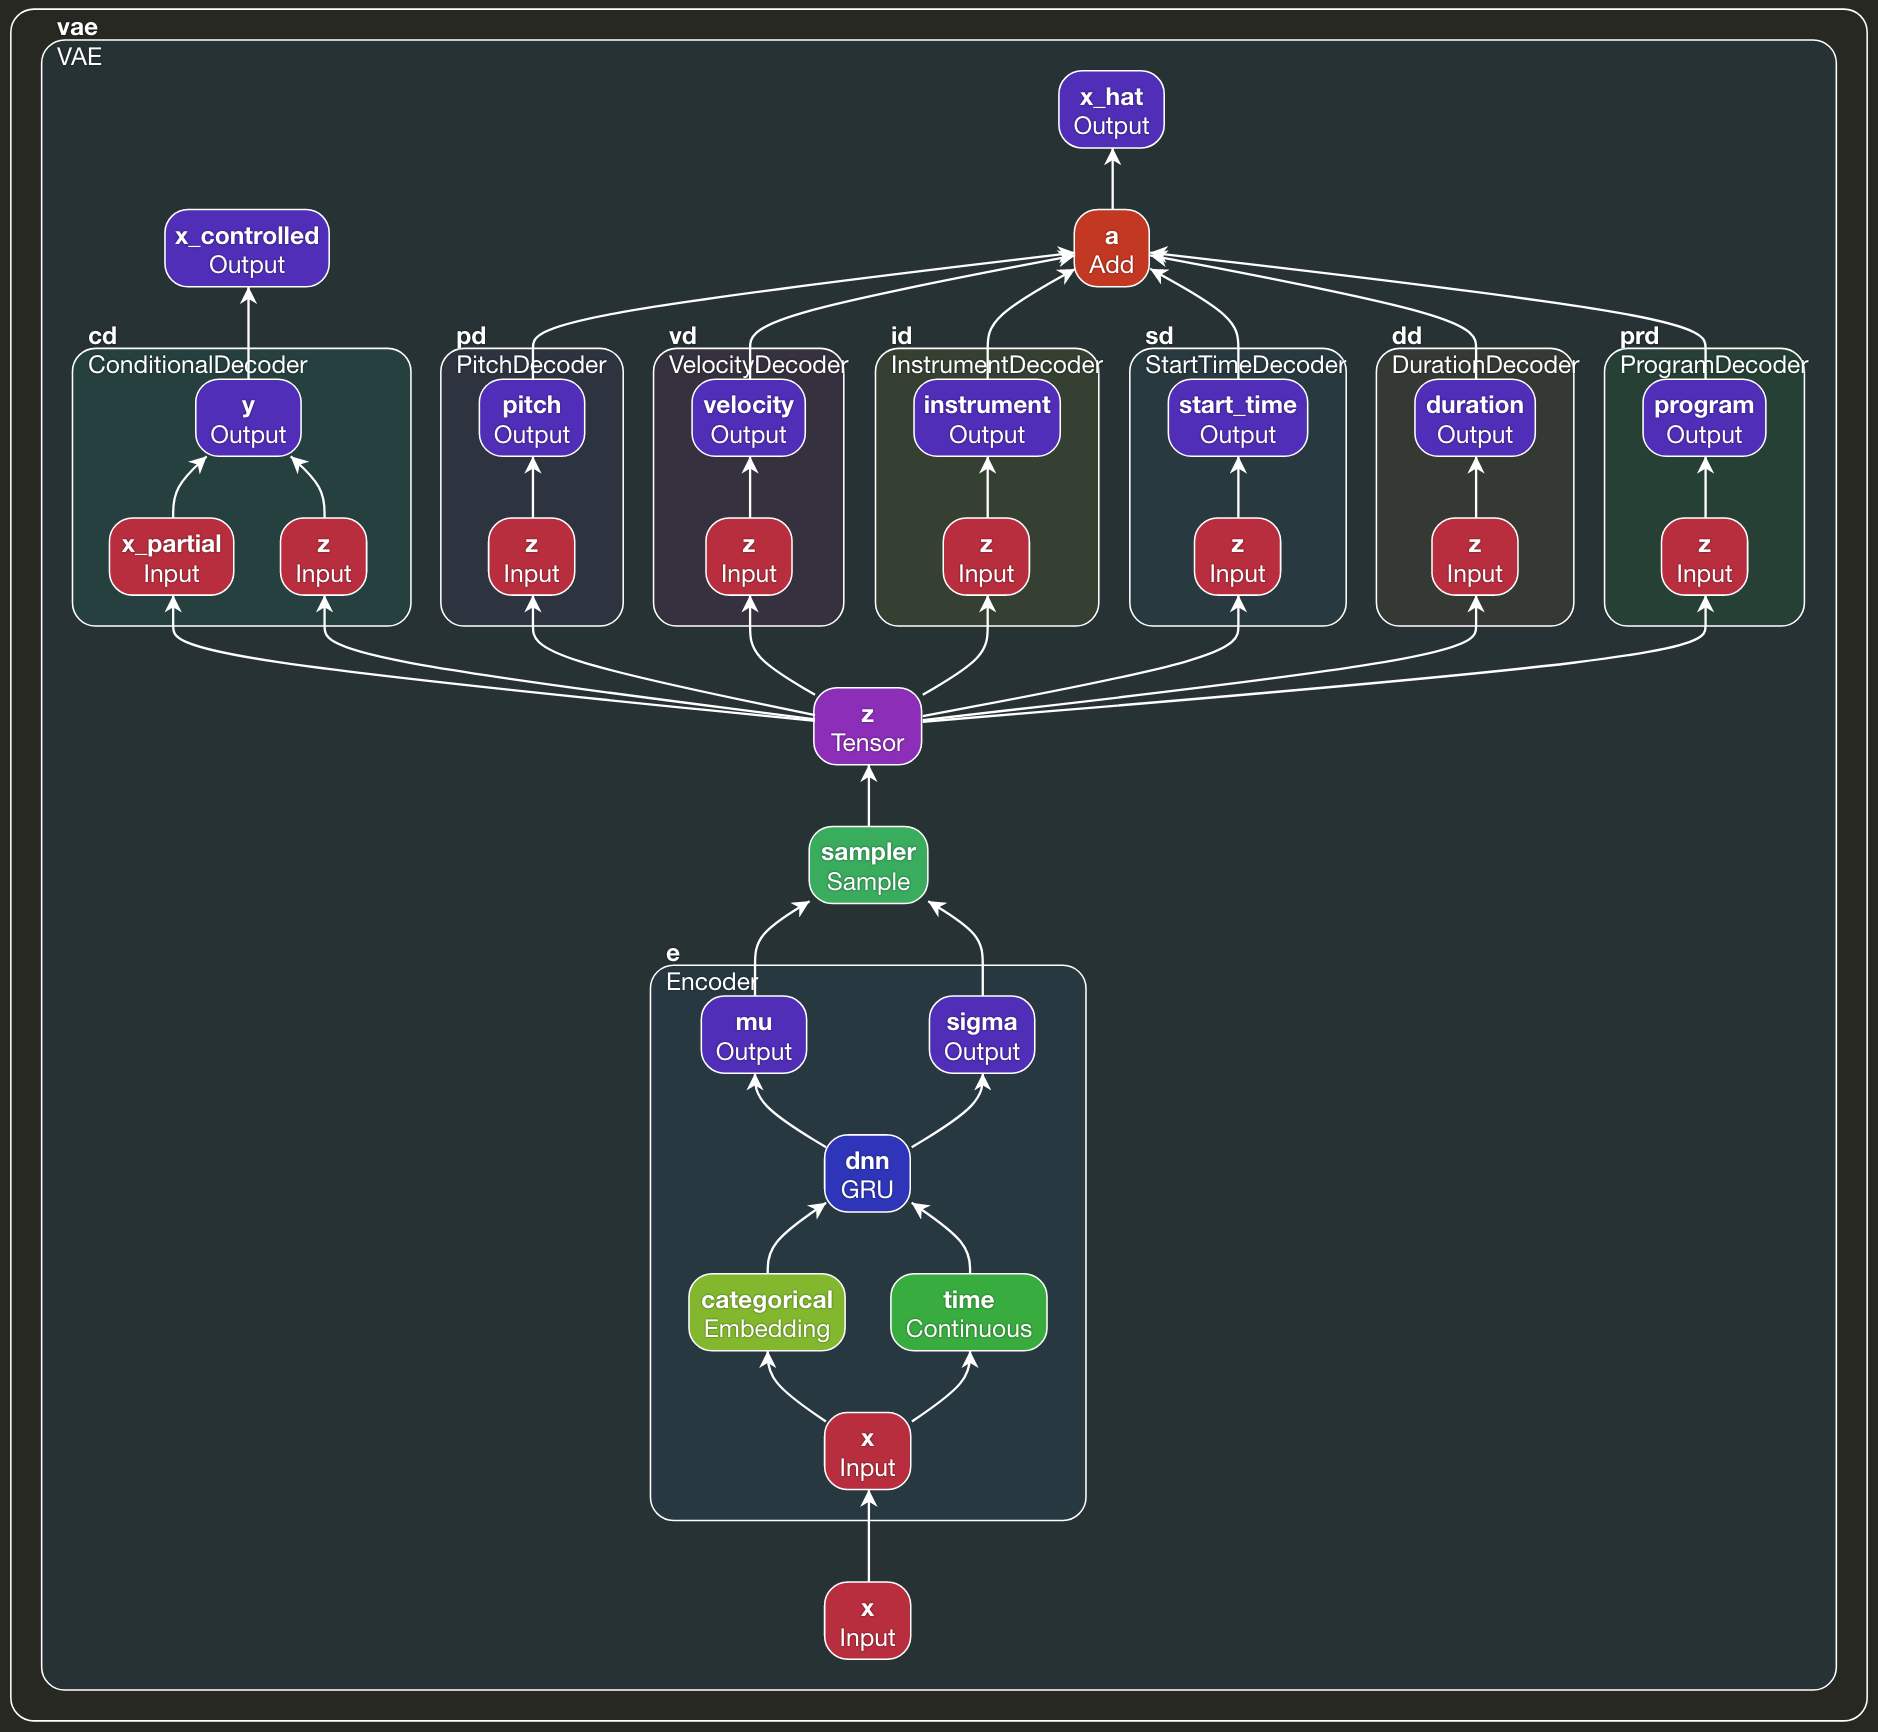
\includegraphics[width=20cm]{midi_vae.png}
\caption{Conditional VAE Architecture}
\end{figure}

\end{block}


\begin{block}{VAE Architecture}

Considerations:

\begin{itemize}
\item Variables Pitch, Velocity, Instrument and Program are categorical variables.
\item Variables Start time and End time are continuous.
\item Hence we need different decoders for Categorical and Continuous variables.
\item A separate decoder for controlled music generation.
\item One-hot encoding cannot be used for categorical variables - Memory usage.
\end{itemize}

We convert the categorical variables to embedding space and use this representation in training. To decode back to categorical values, we check closes $L1$ distance of the \textbf{logits} to each of the embedding weights. The embeddings are learned during training and allow a much smaller memory foot print.
 


\end{block}
%----------------------------------------------------------------------------------------

\end{column} % End of column 2.1

\begin{column}{\onecolwid}\vspace{-.6in} % The second column within column 2 (column 2.2)

%----------------------------------------------------------------------------------------
%	METHODS
%----------------------------------------------------------------------------------------

\begin{block}{Loss}


The total loss in our Architecture is a sum of $KL$ loss, categorical cross entropy losses, reconstruction losses and controlled reconstruction loss:
$$ \mathbb{E}_{q_{\phi}(z|x_{time})} [ \log(p_{\theta}(x_{time}|z))]  - \mathbb{D}(q_{\phi}(z|x) || p(z)) $$
$$ +~\mathbb{E}_{q_{\phi}(z|x_{duration})} [ \log(p_{\theta}(x_{time}|z))] $$
$$ +~\mathbb{E}_{q_{\phi}(z|x,x_{partial})} [ \log(p_{\theta}(x|z, x_{partial}))] $$
$$ -~\mathbb{D}(q_{\phi}(z|x, x_{partial}) || p(z)) $$
$$ +~ \mathbb{E}_{q_{\phi}(z|x,x_{partial})} [ \log(p_{\theta}(x|z, x_{partial}))] $$
$$ -~ \mathbb{D}(q_{\phi}(z|x, x_{partial}) || p(z)) $$
$$ -~\sum_{i=1}^{128} x_{pitch} \cdot \mathrm{log}\; {\hat{x}}_{pitch} $$
$$ -~\sum_{i=1}^{128} x_{velocity} \cdot \mathrm{log}\; {\hat{x}}_{velocity} $$
$$ -~\sum_{i=1}^{128} x_{instruments} \cdot \mathrm{log}\; {\hat{x}}_{instruments} $$
$$ -~\sum_{i=1}^{128} x_{program} \cdot \mathrm{log}\; {\hat{x}}_{program} $$

\end{block}

%----------------------------------------------------------------------------------------


\begin{alertblock}{Generated Sample}


\begin{figure}
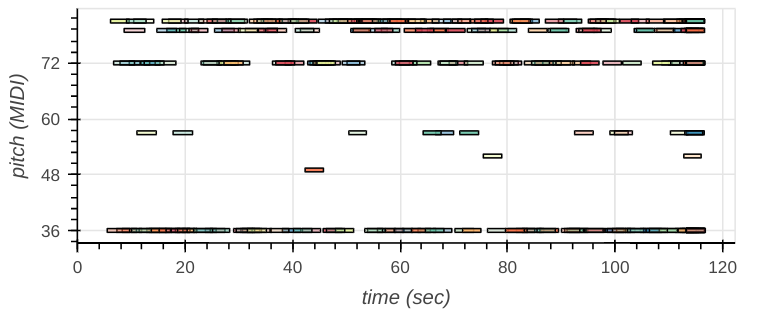
\includegraphics[width=0.9\linewidth]{winter_planet_midi_plot.png}
\caption{Pitch and Velocity Plot of Generated Sample}
\end{figure}

The generated samples follow patterns found in the MIDI files. In this case one can see repeated patterns, a small number of instruments and varying velocity levels in the plot. This sample can be listened at \href{https://soundcloud.com/saravana-r-389436812/cs236-multi-instrument-music-generation-using-vae?si=53eaea6cb734413d80f88bcabc25d3c4}{\textit{SoundCloud Link}}

\end{alertblock} 

\end{column} % End of column 2.2

\end{columns} % End of the split of column 2 - any content after this will now take up 2 columns width

%----------------------------------------------------------------------------------------
%	IMPORTANT RESULT
%----------------------------------------------------------------------------------------

%----------------------------------------------------------------------------------------

\begin{columns}[t,totalwidth=\twocolwid] % Split up the two columns wide column again

\begin{column}{\onecolwid} % The first column within column 2 (column 2.1)

%----------------------------------------------------------------------------------------
%	MATHEMATICAL SECTION
%----------------------------------------------------------------------------------------



%----------------------------------------------------------------------------------------

\end{column} % End of column 2.1

\begin{column}{\onecolwid} % The second column within column 2 (column 2.2)

%----------------------------------------------------------------------------------------
%	RESULTS
%----------------------------------------------------------------------------------------

%----------------------------------------------------------------------------------------

\end{column} % End of column 2.2

\end{columns} % End of the split of column 2

\end{column} % End of the second column

\begin{column}{\sepwid}\end{column} % Empty spacer column

\begin{column}{\onecolwid} % The third column

%----------------------------------------------------------------------------------------
%	CONCLUSION
%----------------------------------------------------------------------------------------

\begin{block}{Results}

The losses in the simple VAE case did not converge. The beta VAE trained models did not produce good quality audio output. The model learned to produce related musical instruments together and have repeated variations in background audio. The pitch and velocity of many samples did not feel like noise. However the results seem to be affected by class imbalance of the input, which has a lot of Piano music and less of other types of instruments.

\begin{figure}
    \centering
    \subfloat[\centering Test Loss]{{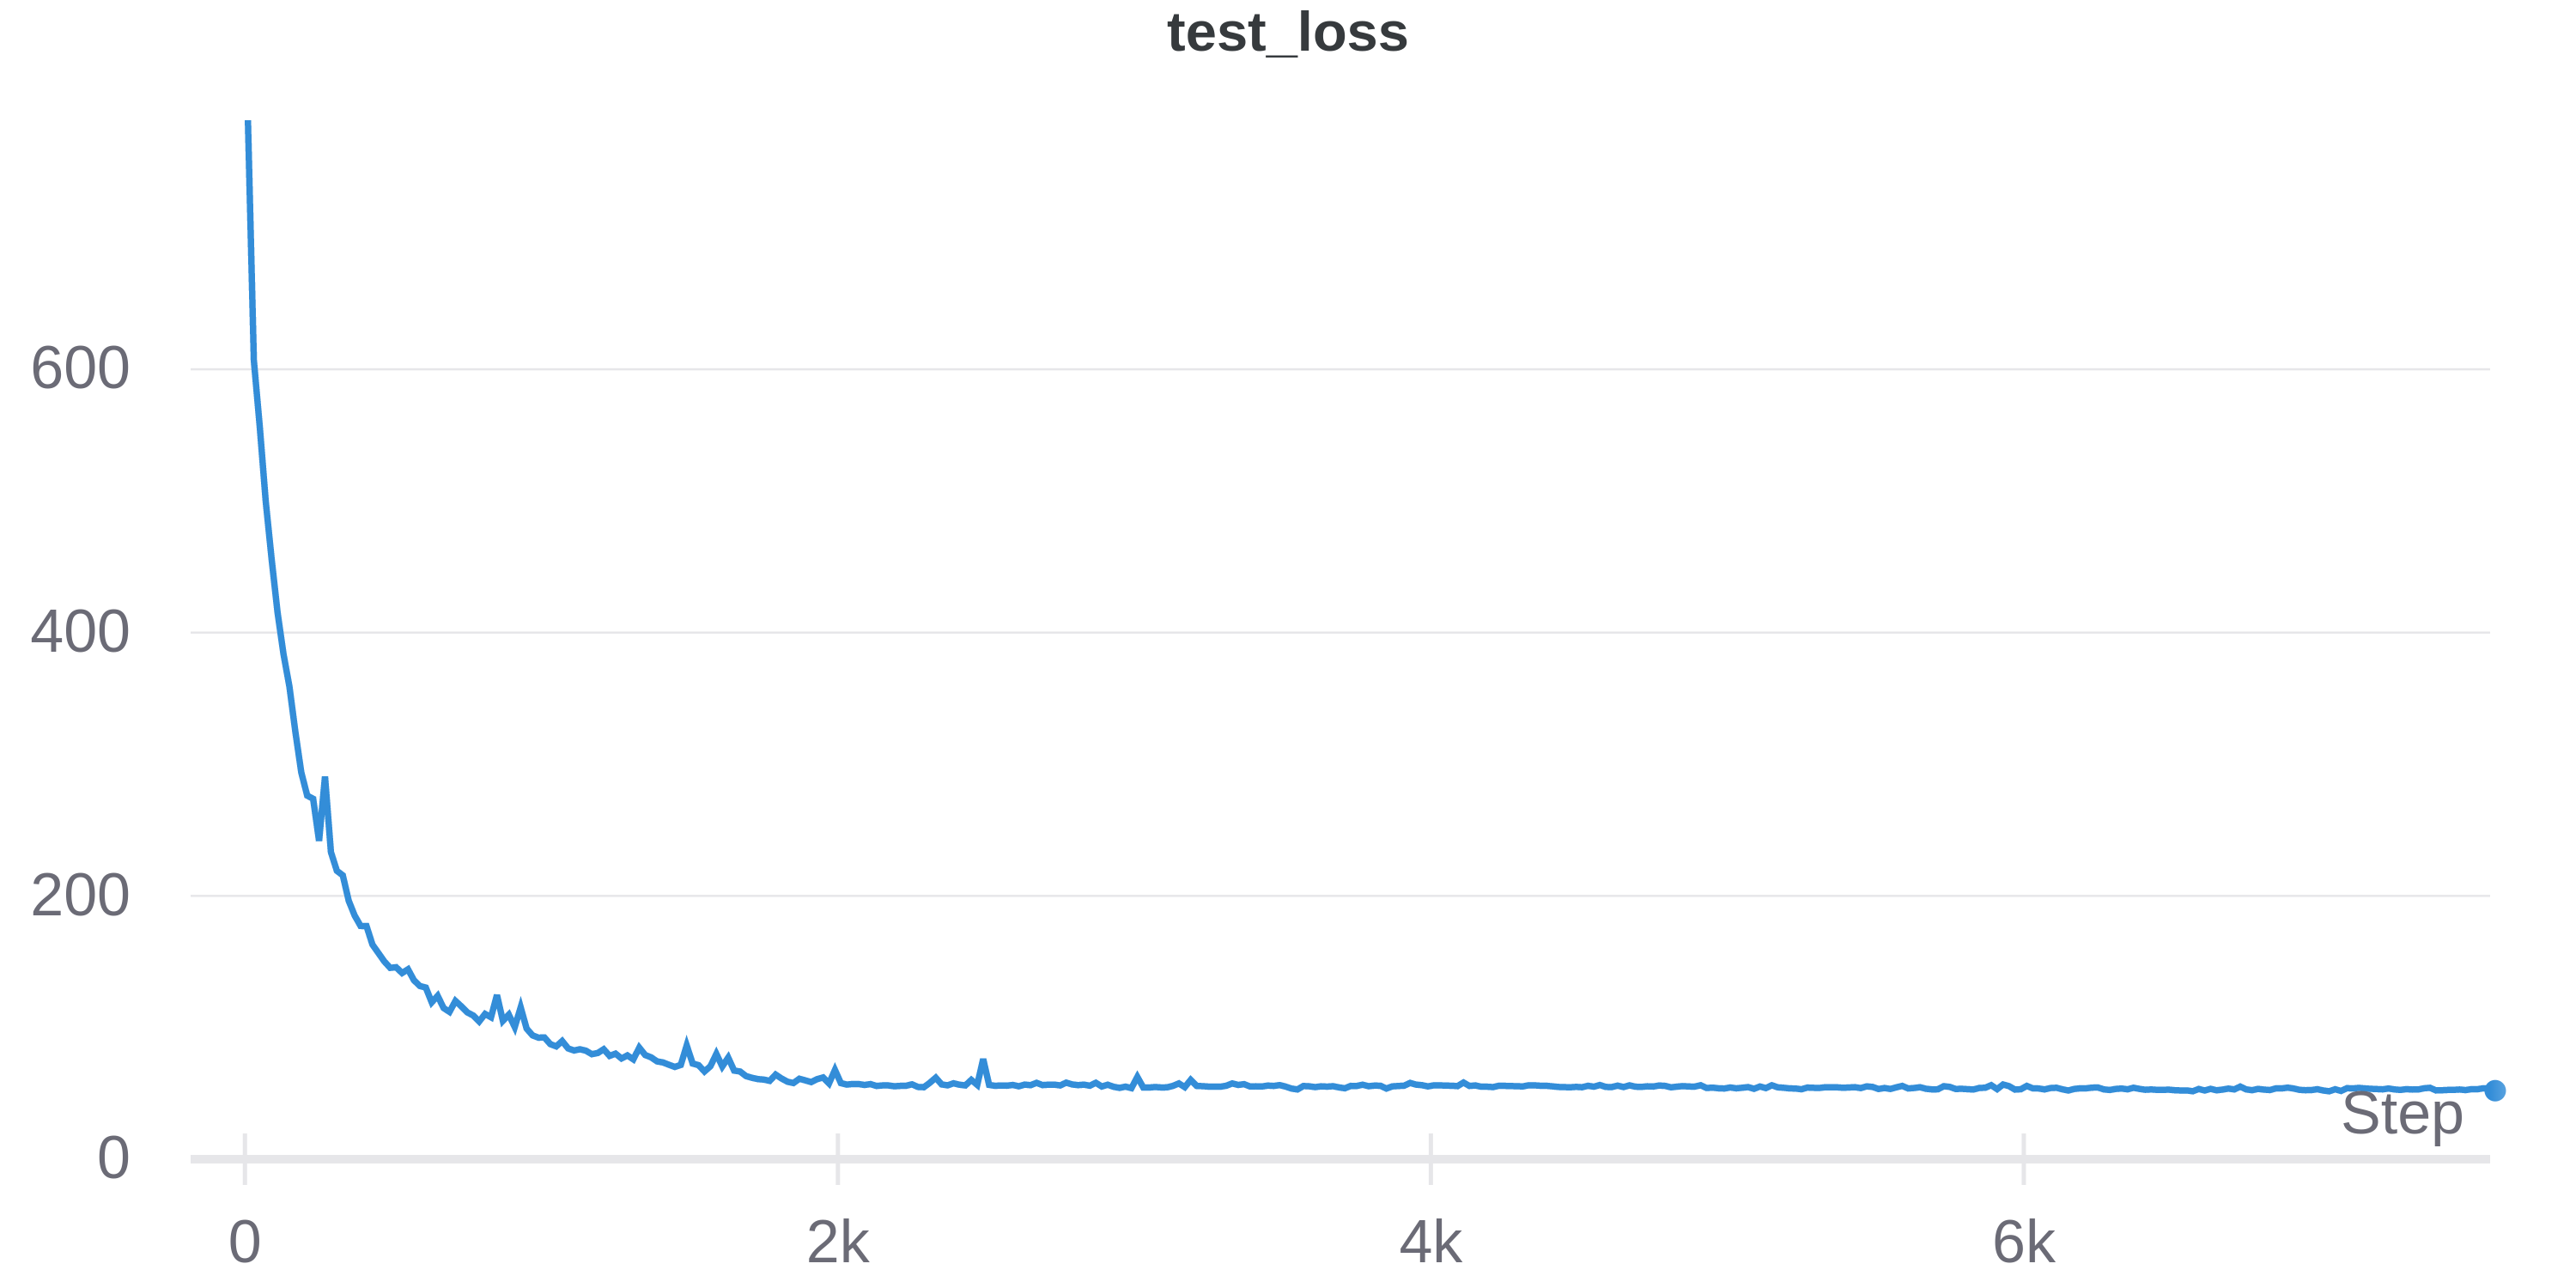
\includegraphics[width=12cm]{testloss.png} }}% 
    \qquad
    \subfloat[\centering Train Loss]{{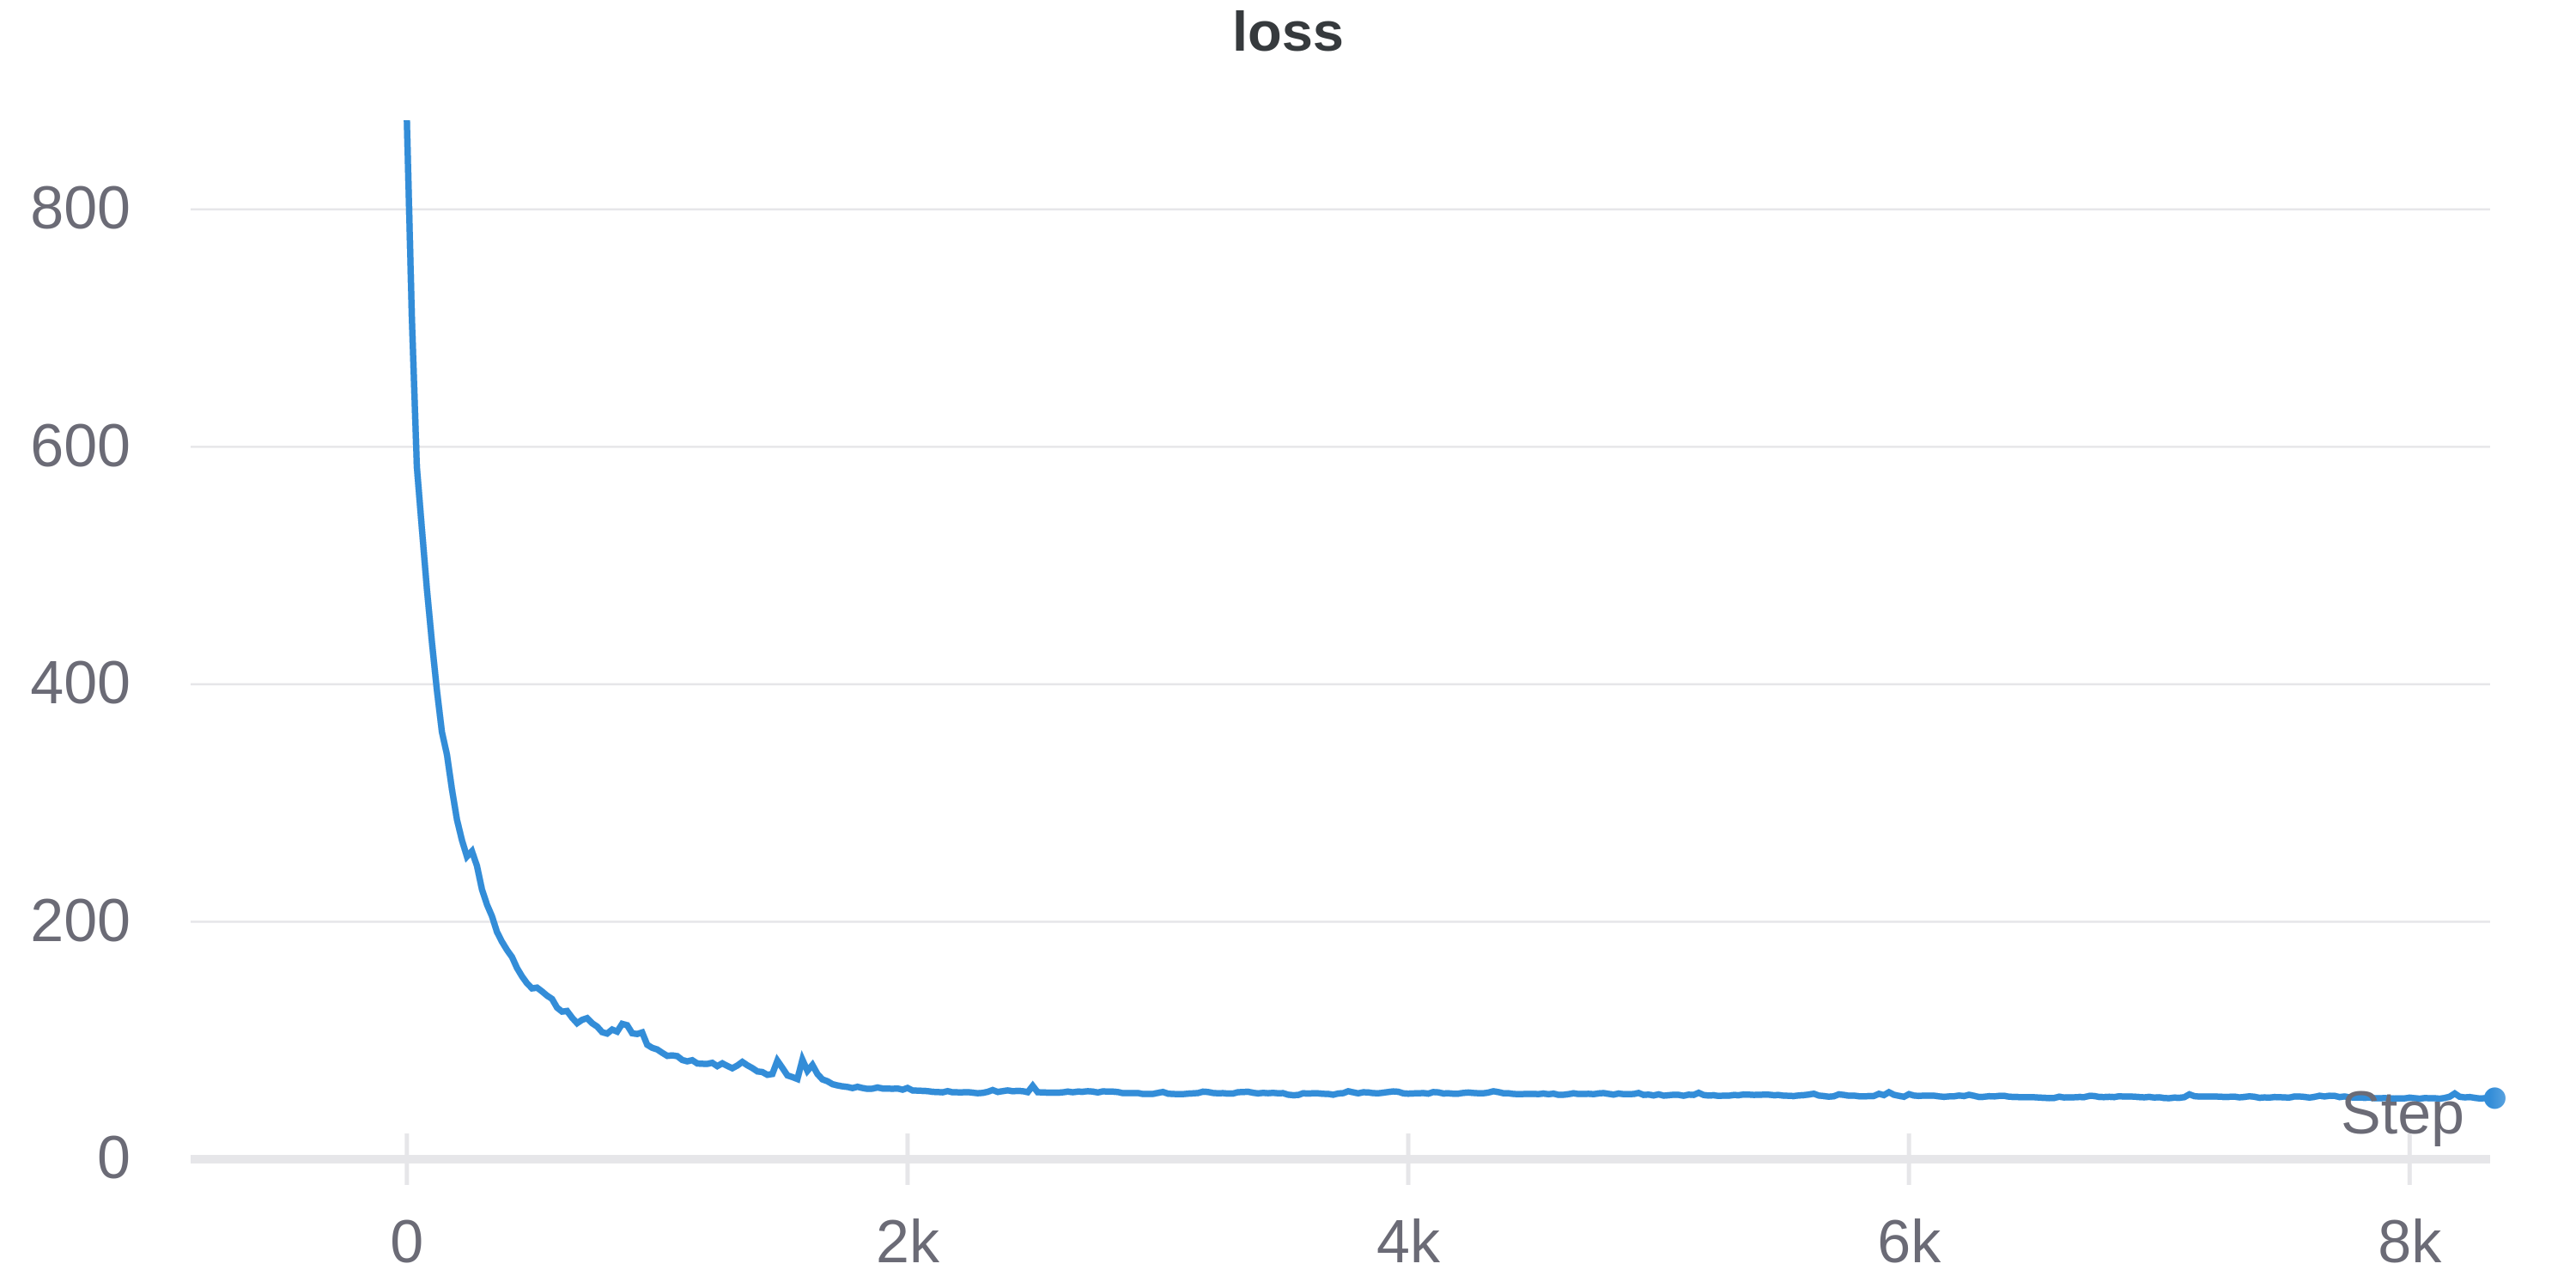
\includegraphics[width=12cm]{train_loss.png}}}%
    \caption{Test and Train Loss}%
\end{figure}


\end{block}

%----------------------------------------------------------------------------------------
%	ADDITIONAL INFORMATION
%----------------------------------------------------------------------------------------

\begin{block}{Acknowledgements}

My TA mentor, \textbf{Kelly He} is awesome! Thank you Kelly. This project would not be possible without your prompt guidance and support. And thank you \textbf{Jiaming Song}, \textbf{Chenlin Meng} and \textbf{Kristy Choi} for the very thoughtful discussions, ideation and support on building this project.


\end{block}

%----------------------------------------------------------------------------------------
%	REFERENCES
%----------------------------------------------------------------------------------------

\begin{block}{References}
\nocite{*} % Insert publications even if they are not cited in the poster
\small{\bibliographystyle{unsrt}
\bibliography{sample}\vspace{0.25in}}
\end{block}

%----------------------------------------------------------------------------------------
%	ACKNOWLEDGEMENTS
%----------------------------------------------------------------------------------------


%----------------------------------------------------------------------------------------

\end{column} % End of the third column

\end{columns} % End of all the columns in the poster

\end{frame} % End of the enclosing frame

\end{document}
